\documentclass{anstrans}




%%%% packages and definitions (optional)
\usepackage{graphicx} % allows inclusion of graphics
\usepackage{graphics}
\usepackage{booktabs} % nice rules (thick lines) for tables
\usepackage{microtype} % improves typography for PDF



\newcommand{\SN}{S$_N$}
\renewcommand{\vec}[1]{\bm{#1}} %vector is bold italic
\newcommand{\vd}{\bm{\cdot}} % slightly bold vector dot
\newcommand{\grad}{\vec{\nabla}} % gradient
\newcommand{\ud}{\mathop{}\!\mathrm{d}} % upright derivative symbol
\graphicspath{ {images/} }

\title{Benefits of Siting a Borehole Repository on Non-Operating Nuclear 
Facility - A Summary}
\author{Jin Whan Bae, William Roy, Kathryn Huff}

\institute{\underline{}
Dept. of Nuclear, Plasma, and Radiological Engineering, University of Illinois at Urbana-Champaign
\and
Urbana, IL
}
\email{jbae11@illinois.edu}


%%%% Acronym support

\usepackage[acronym,toc]{glossaries}
%\newacronym{<++>}{<++>}{<++>}
\newacronym[longplural={metric tons of heavy metal}]{MTHM}{MTHM}{metric ton of heavy metal}
\newacronym{ABM}{ABM}{agent-based modeling}
\newacronym{ACDIS}{ACDIS}{Program in Arms Control \& Domestic and International Security}
\newacronym{AHTR}{AHTR}{Advanced High Temperature Reactor}
\newacronym{ANDRA}{ANDRA}{Agence Nationale pour la gestion des D\'echets RAdioactifs, the French National Agency for Radioactive Waste Management}
\newacronym{ANL}{ANL}{Argonne National Laboratory}
\newacronym{API}{API}{application programming interface}
\newacronym{ARE}{ARE}{Aircraft Reactor Experiment}
\newacronym{ARFC}{ARFC}{Advanced Reactors and Fuel Cycles}
\newacronym{ASME}{ASME}{American Society of Mechanical Engineers}
\newacronym{ATWS}{ATWS}{Anticipated Transient Without Scram}
\newacronym{BDBE}{BDBE}{Beyond Design Basis Event}
\newacronym{BIDS}{BIDS}{Berkeley Institute for Data Science}
\newacronym{CAFCA}{CAFCA}{ Code for Advanced Fuel Cycles Assessment }
\newacronym{CDTN}{CDTN}{Centro de Desenvolvimento da Tecnologia Nuclear}
\newacronym{CEA}{CEA}{Commissariat \`a l'\'Energie Atomique et aux \'Energies Alternatives}
\newacronym{CI}{CI}{continuous integration}
\newacronym{CNEN}{CNEN}{Comiss\~{a}o Nacional de Energia Nuclear}
\newacronym{CNERG}{CNERG}{Computational Nuclear Engineering Research Group}
\newacronym{COSI}{COSI}{Commelini-Sicard}
\newacronym{COTS}{COTS}{commercial, off-the-shelf}
\newacronym{CSNF}{CSNF}{commercial spent nuclear fuel}
\newacronym{CTAH}{CTAHs}{Coiled Tube Air Heaters}
\newacronym{CUBIT}{CUBIT}{CUBIT Geometry and Mesh Generation Toolkit}
\newacronym{CURIE}{CURIE}{Centralized Used Fuel Resource for Information Exchange}
\newacronym{DAG}{DAG}{directed acyclic graph}
\newacronym{DANESS}{DANESS}{Dynamic Analysis of Nuclear Energy System Strategies}
\newacronym{DBE}{DBE}{Design Basis Event}
\newacronym{DESAE}{DESAE}{Dynamic Analysis of Nuclear Energy Systems Strategies}
\newacronym{DHS}{DHS}{Department of Homeland Security}
\newacronym{DOE}{DOE}{Department of Energy}
\newacronym{DRACS}{DRACS}{Direct Reactor Auxiliary Cooling System}
\newacronym{DRE}{DRE}{dynamic resource exchange}
\newacronym{DSNF}{DSNF}{DOE spent nuclear fuel}
\newacronym{DYMOND}{DYMOND}{Dynamic Model of Nuclear Development }
\newacronym{EBS}{EBS}{Engineered Barrier System}
\newacronym{EDZ}{EDZ}{Excavation Disturbed Zone}
\newacronym{EIA}{EIA}{U.S. Energy Information Administration}
\newacronym{EPA}{EPA}{Environmental Protection Agency}
\newacronym{EP}{EP}{Engineering Physics}
\newacronym{FCO}{FCO}{Fuel Cycle Options}
\newacronym{FCT}{FCT}{Fuel Cycle Technology}
\newacronym{FEHM}{FEHM}{Finite Element Heat and Mass Transfer}
\newacronym{FEPs}{FEPs}{Features, Events, and Processes}
\newacronym{FHR}{FHR}{Fluoride-Salt-Cooled High-Temperature Reactor}
\newacronym{FLiBe}{FLiBe}{Fluoride-Lithium-Beryllium}
\newacronym{GDSE}{GDSE}{Generic Disposal System Environment}
\newacronym{GDSM}{GDSM}{Generic Disposal System Model}
\newacronym{GENIUSv1}{GENIUSv1}{Global Evaluation of Nuclear Infrastructure Utilization Scenarios, Version 1}
\newacronym{GENIUSv2}{GENIUSv2}{Global Evaluation of Nuclear Infrastructure Utilization Scenarios, Version 2}
\newacronym{GENIUS}{GENIUS}{Global Evaluation of Nuclear Infrastructure Utilization Scenarios}
\newacronym{GPAM}{GPAM}{Generic Performance Assessment Model}
\newacronym{GRSAC}{GRSAC}{Graphite Reactor Severe Accident Code}
\newacronym{GUI}{GUI}{graphical user interface}
\newacronym{HLW}{HLW}{high level waste}
\newacronym{HPC}{HPC}{high-performance computing}
\newacronym{HTC}{HTC}{high-throughput computing}
\newacronym{HTGR}{HTGR}{High Temperature Gas-Cooled Reactor}
\newacronym{IAEA}{IAEA}{International Atomic Energy Agency}
\newacronym{IEMA}{IEMA}{Illinois Emergency Mangament Agency}
\newacronym{INL}{INL}{Idaho National Laboratory}
\newacronym{IPRR1}{IRP-R1}{Instituto de Pesquisas Radioativas Reator 1}
\newacronym{IRP}{IRP}{Integrated Research Project}
\newacronym{ISFSI}{ISFSI}{Independent Spent Fuel Storage Installation}
\newacronym{ISRG}{ISRG}{Independent Student Research Group}
\newacronym{JFNK}{JFNK}{Jacobian-Free Newton Krylov}
\newacronym{LANL}{LANL}{Los Alamos National Laboratory}
\newacronym{LBNL}{LBNL}{Lawrence Berkeley National Laboratory}
\newacronym{LCOE}{LCOE}{levelized cost of electricity}
\newacronym{LDRD}{LDRD}{laboratory directed research and development}
\newacronym{LFR}{LFR}{Lead-Cooled Fast Reactor}
\newacronym{LLNL}{LLNL}{Lawrence Livermore National Laboratory}
\newacronym{LMFBR}{LMFBR}{Liquid Metal Fast Breeder Reactor}
\newacronym{LOFC}{LOFC}{Loss of Forced Cooling}
\newacronym{LOHS}{LOHS}{Loss of Heat Sink}
\newacronym{LOLA}{LOLA}{Loss of Large Area}
\newacronym{LP}{LP}{linear program}
\newacronym{MA}{MA}{minor actinide}
\newacronym{MCNP}{MCNP}{Monte Carlo N-Particle code}
\newacronym{MILP}{MILP}{mixed-integer linear program}
\newacronym{MIT}{MIT}{the Massachusetts Institute of Technology}
\newacronym{MOAB}{MOAB}{Mesh-Oriented datABase}
\newacronym{MOOSE}{MOOSE}{Multiphysics Object-Oriented Simulation Environment}
\newacronym{MOX}{MOX}{mixed oxide}
\newacronym{MSBR}{MSBR}{Molten Salt Breeder Reactor}
\newacronym{MSRE}{MSRE}{Molten Salt Reactor Experiment}
\newacronym{MSR}{MSR}{Molten Salt Reactor}
\newacronym{NAGRA}{NAGRA}{National Cooperative for the Disposal of Radioactive Waste}
\newacronym{NEAMS}{NEAMS}{Nuclear Engineering Advanced Modeling and Simulation}
\newacronym{NEUP}{NEUP}{Nuclear Energy University Programs}
\newacronym{NFCSim}{NFCSim}{Nuclear Fuel Cycle Simulator}
\newacronym{NGNP}{NGNP}{Next Generation Nuclear Plant}
\newacronym{NMWPC}{NMWPC}{Nuclear MW Per Capita}
\newacronym{NNSA}{NNSA}{National Nuclear Security Administration}
\newacronym{NPRE}{NPRE}{Department of Nuclear, Plasma, and Radiological Engineering}
\newacronym{NQA1}{NQA-1}{Nuclear Quality Assurance - 1}
\newacronym{NRC}{NRC}{Nuclear Regulatory Commission}
\newacronym{NSF}{NSF}{National Science Foundation}
\newacronym{NSSC}{NSSC}{Nuclear Science and Security Consortium}
\newacronym{NUWASTE}{NUWASTE}{Nuclear Waste Assessment System for Technical Evaluation}
\newacronym{NWF}{NWF}{Nuclear Waste Fund}
\newacronym{NWTRB}{NWTRB}{Nuclear Waste Technical Review Board}
\newacronym{OCRWM}{OCRWM}{Office of Civilian Radioactive Waste Management}
\newacronym{ORION}{ORION}{ORION}
\newacronym{ORNL}{ORNL}{Oak Ridge National Laboratory}
\newacronym{PARCS}{PARCS}{Purdue Advanced Reactor Core Simulator}
\newacronym{PBAHTR}{PB-AHTR}{Pebble Bed Advanced High Temperature Reactor}
\newacronym{PBFHR}{PB-FHR}{Pebble-Bed Fluoride-Salt-Cooled High-Temperature Reactor}
\newacronym{PEI}{PEI}{Peak Environmental Impact}
\newacronym{PH}{PRONGHORN}{PRONGHORN}
\newacronym{PRKE}{PRKE}{Point Reactor Kinetics Equations}
\newacronym{PSPG}{PSPG}{Pressure-Stabilizing/Petrov-Galerkin}
\newacronym{PWAR}{PWAR}{Pratt and Whitney Aircraft Reactor}
\newacronym{PWR}{PWR}{Pressurized Water Reactor}
\newacronym{PyNE}{PyNE}{Python toolkit for Nuclear Engineering}
\newacronym{PyRK}{PyRK}{Python for Reactor Kinetics}
\newacronym{QA}{QA}{quality assurance}
\newacronym{RDD}{RD\&D}{Research Development and Demonstration}
\newacronym{RD}{R\&D}{Research and Development}
\newacronym{RELAP}{RELAP}{Reactor Excursion and Leak Analysis Program}
\newacronym{RIA}{RIA}{Reactivity Insertion Accident}
\newacronym{RIF}{RIF}{Region-Institution-Facility}
\newacronym{SFR}{SFR}{Sodium-Cooled Fast Reactor}
\newacronym{SINDAG}{SINDA{\textbackslash}G}{Systems Improved Numerical Differencing Analyzer $\backslash$ Gaski}
\newacronym{SKB}{SKB}{Svensk K\"{a}rnbr\"{a}nslehantering AB}
\newacronym{SNF}{SNF}{spent nuclear fuel}
\newacronym{SNL}{SNL}{Sandia National Laboratory}
\newacronym{STC}{STC}{specific temperature change}
\newacronym{SUPG}{SUPG}{Streamline-Upwind/Petrov-Galerkin}
\newacronym{SWF}{SWF}{Separations and Waste Forms}
\newacronym{SWU}{SWU}{Separative Work Unit}
\newacronym{TRIGA}{TRIGA}{Training Research Isotope General Atomic}
\newacronym{TRISO}{TRISO}{Tristructural Isotropic}
\newacronym{TSM}{TSM}{Total System Model}
\newacronym{TSPA}{TSPA}{Total System Performance Assessment for the Yucca Mountain License Application}
\newacronym{ThOX}{ThOX}{thorium oxide}
\newacronym{UFD}{UFD}{Used Fuel Disposition}
\newacronym{UML}{UML}{Unified Modeling Language}
\newacronym{UOX}{UOX}{uranium oxide}
\newacronym{UQ}{UQ}{uncertainty quantification}
\newacronym{US}{US}{United States}
\newacronym{UW}{UW}{University of Wisconsin}
\newacronym{VISION}{VISION}{the Verifiable Fuel Cycle Simulation Model}
\newacronym{VV}{V\&V}{verification and validation}
\newacronym{WIPP}{WIPP}{Waste Isolation Pilot Plant}
\newacronym{YMR}{YMR}{Yucca Mountain Repository Site}

	
\makeglossaries

%%%%%%%%%%%%%%actual words%%%%%%%%%%%%%%%%%%%%%%%%%%%%%%%%%%%%%%%%%%%%%%%%%%%%5


\begin{document}


%%%%%%%%%%%%%%%%%%%%%%%%%%%%%%%%%%%%%%%%%%%%%%%%%%%%%%%%%%%%%%%%%%%%%%%%%%%%%%%%
\begin{abstract}
This paper is a summarized version of a paper for the \gls{IHLRWM} conference.
This work evaluates a potential solution for two pressing matters in the viability of
nuclear energy: spent fuel disposal and power plants that no longer operate. The 
potential benefits of siting a borehole repository at a shut down nuclear power 
plant facility are analyzed from the perspective of myriad stakeholders. 
This assessment indicates that integrated siting will make economic 
use of the shut down power plant, take advantage of spent fuel handling 
infrastructure at those sites, minimize transportation costs, expedite emptying 
the crowded spent fuel storage pools across the country, and will do so at 
sites more likely to have consenting communities.
\end{abstract}

   \section{Introduction}

This work evaluates the benefits of turning a shutdown reactor,
a liability, to a borehole repository site, a much-needed facility.
This work evaluates a strategy to do so that the remaining facilities
are leveraged to cut costs and time for the repository, which makes
the repository construction and operation more economical and 
politically feasible. 

The  expected benefits of this 
proposed integrated siting strategy include reduced radioactive waste 
transportation burden, increased likelihood of consent from the local 
community, and improved expediency achieved through leveraging existing 
infrastructure and skill.

The proposed case is compared to the case of Yucca Mountain, in six
quantitative measures, in the perspective of four stakeholders.

\subsection{Motivation}
This work suggests borehole-design repositories for such integrated facility due it 
the design's modularity, wide geological suitability, and footprint 
efficiency. Borehole repositories need crystalline basement rocks at 
$ 2,000 - 5,000m$ deep, which is relatively common in the continental 
U.S \cite{arnold_research_2012}. Also, the area required for a 
borehole repository is only $30 km^2$ for the capacity of Yucca Mountain
 \cite{brady_deep_2009}.
 
The pre-existing local talent and infrastructure, is a major
benefit to the proposed design. Compared to Yucca Mountain, where little 
infrastructure existed, a shutdown power plant is more likely to have
usable infrastructure left, which can be utilized to save cost and time.

Lastly, the proposed design allows for more consent-based siting, 
since communities with nuclear facilities are more likely to be 
more receptive to the benefits of hosting a repository (i.e. jobs and taxes). 

The purpose of this paper is to attempt to quantify the benefits, and compare
them to the case of Yucca Mountain through a case study.

   
\section{Case Definitions}

This paper proposes siting a borehole
 repository at a shut down nuclear power plant such as one similar to the 
 Clinton Power Plant in Illinois. This proposed case is then compared to a 
 reference case at Yucca Mountain. 
 
The paper focuses on the benefits that arise from the strategic siting of a repository 
on a non-operating nuclear facility, and not the benefits that arise from the repository design. 
The borehole design follows the Sandia Report Reference Design and Operations 
for Deep Borehole Radioactive Waste \cite{arnold_reference_2011}. Selection of 
an alternative borehole concept could impact the details of the repacking needs 
and facility design, but will not significantly impact the siting comparison 
here.
 
\subsection{Case I: Reference Case} 
The reference case, upon which the proposed case seeks to improve, is to build 
a standalone 70,000 \gls{MTHM} mined repository at the Yucca Mountain site.

The reference case is presented in order to demonstrate the cost savings and efficiencies 
that arise from the proposed case. The base case mimics the Yucca Mountain Project.
Costs include new licensing and processing facility for repacking the spent fuel assemblies.

\subsection{Case II: Shut Down Plant Case}

The imminent shutdown of the Clinton Nuclear Power Station has recently been 
averted by an act of the state legislature. In this sense, Clinton is 
representative of a class of at-risk nuclear 
reactors in the Midwest and eastern United States. A borehole repository 
sited at the Clinton Nuclear Power station site is therefore hypothetically 
considered here to represent integrated repository siting at a reactor facility 
faced with potential shutdown.

The Clinton Nuclear Power Station is owned by the Exelon Corporation. It has a 
licensed land area of approximately $58 km^2$ and a $20 km^2$ cooling heat sink, 
the Clinton Lake. Of the licensed land area, only $0.6 km^2$ is used for the facility.  
\cite{nrc_chapter_2007}.  This leaves enough room left for a 70,000 \gls{MTHM} 
borehole repository without additional land purchase from the public.

\subsection{Potential Plan: Combined Case}
As an aside, given that one 70,000 \gls{MTHM} repository is already insufficient for 
domestic \gls{SNF} needs \cite{doe_report_2008}, a potential plan for the future can be proposed, 
a dual-repository scenario. In this scenario, both the Yucca Mountain 
repository and the near-Clinton borehole repository are sited and someday 
become operational. The proposal that a pair of repositories, east and west, is 
not new. Indeed, it was originally envisioned before the Yucca Mountain site 
selection was made.

In this scheme, eastern reactors send their spent fuel to the eastern 
repository site while western reactors send theirs to the western site. Thus, 
the less-nuclear western region will not bear the burden of hosting a 
repository for the eastern region, which has a larger percent of nuclear 
energy. 

For this scenario, spent fuel west of the 92 west meridian is considered west, 
which will send its \gls{SNF} to Yucca Mountain. Conversely, spent fuel east of the 92 west
meridian is considered east, which will send its \gls{SNF} to the proposed Clinton 
power plant. The 92 west meridian is chosen because it is the meridian just west of
Illinois state borders, so that no Illinois power plants have to transport their
spent fuel to Yucca Mountain. This plan will be analyzed in the paper but should
not be a comparison to the previous two cases because it has different capacities. %no division.


\section{Methodology}

This work will evaluate \textbf{2 scenarios} for repository siting according to \textbf{6 metrics} of 
performance considered from the perspective of \textbf{4 stakeholders.}

Preliminary work \cite{waleed_regional_2015} suggests that integrated siting 
will reduce costs, construction, time (both for construction and licensing), 
transportation distances, and resistance from the local community.  
The goal of this paper is to compare this siting strategy with the 
business-as-usual base case via quantitative metrics capturing the key 
priorities of stakeholders. Accordingly, the present 
work will compare case one and two along these axes. 

%%%%%%%%%%%%%%%%%%%%%%%%%%%%%%%%%%%%%%%%%%%%%%%%%%%%%%%%%%%%%%%%%%%
\iffalse

\begin{itemize}
	\item The reference case: a standalone borehole repository at Yucca Mountain.  
	\item The proposed case: a repository sited at a shutdown reactor site 
	in the Midwest.


\end{itemize}

\fi

%%%%%%%%%%%%%%%%%%%%%%%%%%%%%%%%%%%%%%%%%%%%%%%%%%%%%%%%%%%%%%%%%%%

This work will evaluate the potential impacts of each siting strategy according 
to the following 6 quantitative measures:

\begin{itemize}
	\item Transportation Burden $[MTHM \cdot km]$: A site is preferred by 
	most stakeholders if it can minimize the distance \gls{SNF} 
	must travel.
	\item Workforce Utilization $[-]$: A repository site is preferred by 
	many stakeholders if it utilizes an already situated skilled local 
	workforce. 
	\item Expediency $[y]$: Many stakeholders will benefit if the removal 
	of dry casks from current storage pads is expedited.
	\item Consent Basis $[\frac{nuclear MW}{\mbox{capita}}]$: If the community
	 beneifts from nuclear energy, they are more likely to be consenting to
	 site a repository. If there is a basis for a consent-based 
	siting process to succeed, many stakeholders benefit.
	\item Site Access $[-]$: Rail access to the site is essential for 
	beginning operations.
	\item Site Appropriateness $[-]$: A site must be geologically 
	appropriate and of sufficient area.
\end{itemize}

Finally, recognizing that these measures are valued differently by each, we
consider possible weighting factors that may capture the perspectives of 4 key
stakeholder groups:

\begin{itemize}
	\item the federal government,
	\item the state government,
	\item the local government / community,
	\item and the owner of the non-operating plant.
\end{itemize}


\section{Evaluation Metrics}

This paper introduces six metrics of siting performance. These metrics and 
their definitions draw upon previous 
\cite{freeze_siting_2015,waleed_regional_2015} as well as original work.  In 
the following sections, the metrics are defined in more detail, and normalized
so that in the final section, they are applied to comparatively evaluate each case.

The normalization of the metrics are done to a scale of 0 to 1 using the equation
below, where 0 is the worst possible value, and 1 the best. 
%If the best case
%value is smaller than the worst case value, the numerator and the denominator is
%reversed.
 Metrics like transportation burden, expediency, and consent basis,
 are normalized in such a matter. Metrics without units are booleans, where values 
 only exist in values of 0 or 1. For example, a 0 value for site access means 
that there is no existing site access infrastructure.


\begin{align} 
	\mbox{NV} &= \frac{x-\mbox{W}}{\mbox{B}-\mbox{W}}\\
	NV &= \mbox{normalized value for the metric}\\
	x &= \mbox{considered case value for the metric}\\
	B &= \mbox{best case value for the metric}\\
	W &= \mbox{worst case value for the metric}\\
\end{align}



\subsection{Transportation Burden}
 In order to minimize transport cost, a central location is preferred. To 
 capture this, a metric 
 for representing the distance a mass of spent fuel must be transported, the 
 transport burden, is introduced. This transportation burden is the product 
 of the \gls{SNF} mass and the distance it has to travel from its current 
 storage location to the proposed repository. This results in a 
 metric in units of $MTHM\cdot km$. 

 To arrive at the transportation burden for each case, a distance analysis was 
 completed using the Haversine formula \cite{shumaker_astronomical_1984}. 
 First, the coordinates of each power plant were obtained by scraping public 
 data \cite{nuclear_regulatory_commission_nrc:_2016}.  The distance between each storage site (i.e. reactors 
 and \gls{ISFSI}) was then calculated by using the Haversine formula on the 
 geographical coordinates of the receiving and sending sites (1 and 2). 

 \begin{align} 
         \Phi_1,\Phi_2&= \mbox{latitude in radians}\\
         \lambda_1,\lambda_2 &= \mbox{longitude in radians}\\
         \Delta\lambda &= \left|\lambda_1 - \lambda_2\right|\\
         \Delta\Phi &= \left|\Phi_1 - \Phi_2\right|\\
         a&=\sin^2(\Delta\Phi)+\cos(\Phi_1)\cos(\Phi_2)\sin^2{\left(\frac{\Delta\lambda}{2}\right)}\\
         c &= 2 \cdot arctan2(\sqrt{a},\sqrt{1-a})\\
         d &=  (6,371km) \cdot c
 \end{align}

\begin{align}
        b_i &= m_id\\
        B &= \sum_i^N b_i\\
        \intertext{where}
        b_i &= \mbox{spent fuel transport burden from facility i}\\
        m_i &= \mbox{mass of spent fuel at facility i}\\
        B &= \mbox{total spent fuel transport burden}\\
        N &= \mbox{total number of facilities with spent fuel on site.}
\end{align}

This analysis used GC-859 spent fuel inventory data available from \gls{EIA} 
through private communication \cite{domenico_GC-859_2016} as well as \gls{CURIE}, a web interface to 
the \gls{ORNL} universal database\cite{ornl_centralized_2016}.
From the list of 74 sites, several candidates which minimize $B [MTHM\cdot 
km]$, spent fuel transportation burden, are listed in Table 1.
    
    \begin{table}[h]
    	\centering
    	
    	\caption {Reactors with relatively small spent fuel transportation burden $ [MTHM\cdot km]$.}
    	\scalebox{0.86}{
    		\begin{tabular}{|c|c|c|c|}
    			\hline
    			Reactor & State & $MTHM*km$ & License Area [$km^2$]  \\ \hline
    			Clinton & Illinois &  \textbf{77,352,339} & \textbf{57.87}   \\ \hline
    			Dresden & Illinois &  \textbf{77,663,969} & 3.856   \\ \hline
    			Peach Bottom & Pennsylvania & 85,563,135 & 2.509   \\ \hline
    			Indian Point &   New York & 84,097,374 & .967   \\ \hline
    			Yucca Mountain & Nevada & 209,575,157 & N/A \\ \hline
    			
    		\end{tabular}}
    		\end {table}


%Transitional Section and discussion on Yucca


The Clinton Power Plant was chosen as the site for the proposed case due to its
small $MTHM\cdot km$ value and substantially large license 
area\cite{nrc_chapter_2007}.
Considering that only
$30 km^2$ is required for all the total \gls{SNF} amount, the licensed area at Clinton
power plant allows more than  enough space to site a borehole repository, which
avoids possible conflicts with the community from purchasing and utilizing more
land. 

The proposed case would require enormous cooperation from the utility that owns
the power plant. In the case of Clinton, that would be Exelon Corporation. 
Were Clinton facing shutdown, Exelon would have a strong incentive to 
cooperate in order to utilize the facility property
in a lucrative manner. In particular, Exelon would be able to save on decommissioning of
Clinton by selling the property as well as the infrastructure to the 
government. Though the reactor facility may need to be decommissioned, 
this responsibility could be transferred to the federal government (or 
an independent \gls{SNF} management agency \cite{ayers_blue_2012}) upon 
purchase of the land.

Also, with recent events, the possibility of Yucca Mountain Repository's revival
is on the rise. This brings a potential combined case, where the new
borehole repository will operate with the Yucca Mountain Repository. 

However, partitioning west and east with respect to the 92 west meridian yields the Yucca
Mountain Repository site approximately 
$14,000 [MTHM]$ of \gls{SNF}, much less than its proposed capacity of 70,000 \gls{MTHM}. On the other hand, 
the Clinton repository \gls{SNF} burden would be reduced to 61,777 \gls{MTHM}. The transportation burden is 
$53,945,200 [MTHM\cdot km]$  
for Yucca Mountain, and $17,940,959 MTHM\cdot km$ for the Clinton repository. This 
adds up to a sum of $71,886,160 MTHM\cdot km$, which is about 7\% less than that
of Clinton repository alone. This does not provide a comparable advantage. Other
reactor sites were tested in the transportation burden analysis but also failed
to provide a substantial advantage. Also, the selection of potential sites
was limited by the geological constraints shown in Figure 2.

If the power total MTHM value were to be equal, a line can be drawn at the 84 west
meridian, which yields $39,942 MTHM$ for the east repository, and $36,649 MTHM$ for
the Yucca Mountain repository. One of the original candidates, the Peach Bottom
reactor in Pennsylvania is then chosen for its central location in the east area.
However, this analysis yields a $MTHM\cdot km$ value of $92,575,081 MTHM\cdot km$,
which is substantially larger than that of having one repository in Clinton. 
Also, the Peach Bottom reactor site has little licensed land, which will require
additional land purchase for the repository. 


\begin{table}[h]
	\centering
        \caption {Transportation Burden for Each Case}
	%\scalebox{0.60}{
		\begin{tabular}{|c|c|c|}
			\hline
			Case & Transportation Burden [$MTHM\cdot km$] & NV\\
			\hline
			Case I & 209,575,157  & 0\\
			Case II & 77,352,339 & 1 \\
                        \hline
                \end{tabular}
                %}
\end{table}
  

 \subsection{Site Appropriateness} 

  To host a borehole repository, the site must satisfy geologic requirements. 
  Figure \ref{fig:cbrock} is a map indicating the geological fitness of various 
  regions of the United States. The proposed site at Clinton sits above 
  a crystalline basement which lies at an appropriate depth.

\begin{figure}[!h] 
  \centering
  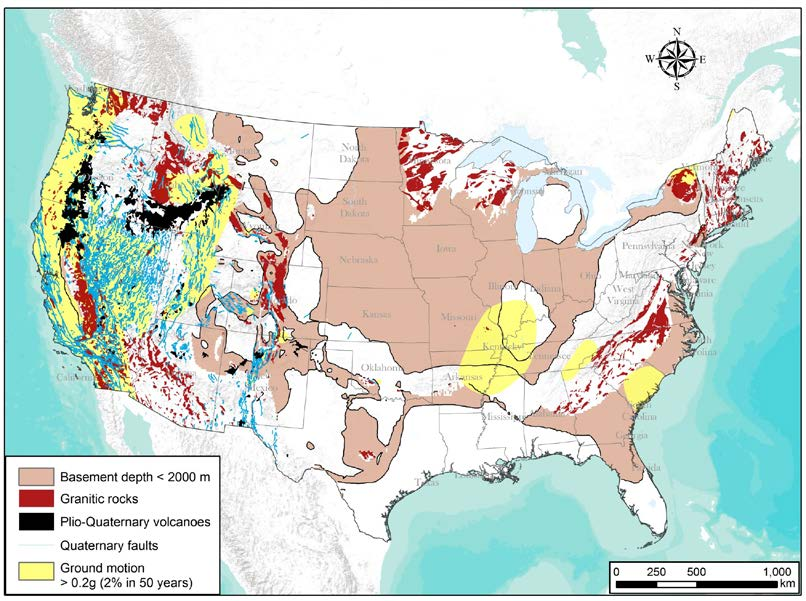
\includegraphics[width=0.8\columnwidth]{cbrock.png}	
        \caption{From \cite{perry_gis_2015}, a map of areas in the US with 
        crystalline basement rock at less than 2000 meters depth. Tectonic 
        activity impacting siting considerations are also mapped:  Quaternary 
        faulting, volcanism, and seismic hazard (yellow shading = 2\% 
        probability of exceeding 0.2 g of ground acceleration in 50 years).}
  \label{fig:cbrock}
\end{figure}

    
  
  Also, it should be noted that the Clinton area is a well studied geologic 
  host area. Ample data on the stratigraphy of the Decatur region, such as  
  Figure \ref{fig:Stratigraphy} has already been collected as part of the 
  Decatur Carbon Sequestration Project which is less than 50 miles south of the 
  Clinton power plant.
 
\begin{figure}[!h] 
  \centering
  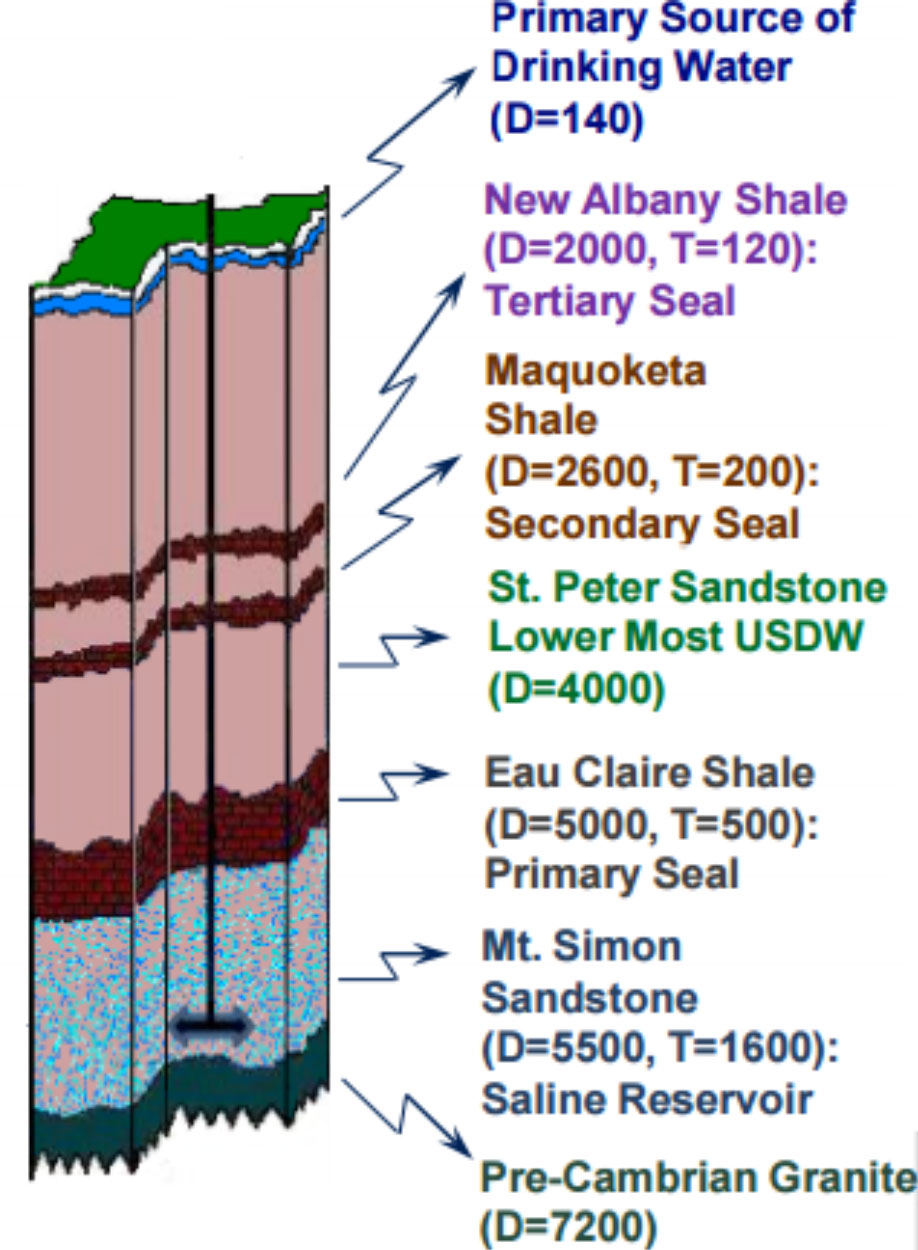
\includegraphics[width=0.8\columnwidth]{Stratigraphy-Decatur}	
  \caption{Stratigraphy of the Decatur Region, D is depth in feet.
  \cite{mcdonald_illinois_2012}.}
 \label{fig:Stratigraphy}
  	
 
\end{figure}
  
\begin{table}[h]
	\centering
        \caption {Site Appropriateness for Each Case}
	%\scalebox{0.60}{
		\begin{tabular}{|c|c|}
			\hline
			Case & Site Appropriateness \\
			\hline
			Case I & 1 \\
			Case II & 1 \\
			\hline
                \end{tabular}
                %}
\end{table}

\subsection{Workforce Utilization}

Building a spent nuclear fuel repository is no easy task. It is a task that requires
numerous experts and laborers. Also, operating and maintaining a nuclear power plant
requires numerous experts and laborers. In case of the proposed case, the Clinton
 Power Station has approximately 700 employees living in nearby counties with an
additional several hundred contractors during fuel 
outages\cite{exelon_clinton_2016}.
The existing skilled workers and local talent for maintenance, transport and catering
services can be utilized without bringing a whole new group of workers to the 
area \cite{iaea_managing_2008}. Also, the shutdown of Clinton Power Plant would cause a dramatic
loss of jobs in the community. 

The void created by the shutdown of the Clinton plant can be, though not
completely, filled by the new construction of a borehole repository. The construction
will prioritize local hires as an incentive to ease local opposition on repository
 siting. Employment during the operation of Yucca Mountain was estimated to range from
 2,000 to 5,000 jobs, \cite{riddel_economic_2003} which means that the borehole repository
 would at least require half of the workforce for the same capacity. 

Additionally, an estimate by the Illinois State University on fracking the New Albany
Shale in southern Illinois estimated that such a project can create 1,000-47,000 jobs
\cite{loomis_potential_2012}. Translating the workforce to central Illinois and the borehole
project should create somewhere in the low and medium estimate, which is about 10,000
jobs.   

The proposed case has a larger advantage over the base case in the sense that there
are already existing facility in regards to spent fuel handling and worker lodging 
and catering services. 
It is assumed, for the sake of argument, half of the construction cost of the
repacking facility in the base case is used to expand the existing facility in the
proposed case. 


\begin{table}[h]
	\centering
        \caption {Workforce Utilization for Each Case}
	%\scalebox{0.60}{
		\begin{tabular}{|c|c|}
			\hline
			Case & Workforce Utilization \\
			\hline
			Case I & 0 \\
			Case II & 1 \\
			\hline
                \end{tabular}
                %}
\end{table}


\subsection{Consent Basis}

International \gls{SNF} siting experiences have shown that a consent-based
approach to siting a repository is crucial to success
\cite{ayers_blue_2012,doe_designing_2016,jenkins-smith_public_2013,freeze_siting_2015}. 
Furthermore, the Swedish precedent \cite{olsson_experiences_2013} shows that 
municipalities near nuclear facilities
are more likely to volunteer to site a repository in their community.

Because populations local to operating reactor sites are more likely to be 
favorable toward nuclear power, and the proposed integrated siting 
is in an already-nuclear community by design, this siting strategy inherently 
maximizes the local consent basis.

The source of this favorable attitude varies by site. 
The local community is the beneficiary of various economic benefits
including job creation and the substantial property taxes paid by the utility 
toward regional governmental budgets.   In the case of the Clinton Power Plant, 
Exelon pays \$15 million in property taxes each year, which amounts to about 
\$923 per resident in the host Dewitt county \cite{brady-lunny_dewitt_2016}. The plant
also provides a total payroll of more than \$50 million to its workers.
The eventual shutdown of the plant would have caused a dramatic loss of the economic inflow.
It is also speculated that 13,300 jobs would be lost in Illinois after five years 
of plant shutdown \cite{reid_study:_2014}.  

A similar phenomenon might be expected at the state level as well, because 
Illinois generates more nuclear energy than any other U.S.  state with a net 
capacity of 11,441 megawatts in 2010 \cite{eia_state_2012}. Nevada, on the other 
hand, hosts zero nuclear power plants. Thus, it can only be natural for Nevada 
to consider a national repository as an unjust burden, despite economic 
benefits.  

The consent basis, driven by proximity to an operating nuclear plant and 
corresponding greater likelihood to be favorable toward hosting an \gls{SNF} 
repository, should be quantifiable by a measure of the benefit experienced by 
the community.  For simplicity, we quantify the proximity to nuclear energy at 
the state level  based on power consumed. The corresponding state and regional 
metrics (expressed in MW of nuclear power per capita) are listed in Table V. This 
analysis uses nuclear power generation capacity and population data from the 
U.S. \gls{EIA} \cite{eia_state_2012} and the U.S. Census \cite{census}.  

\begin{table}[h]
	
	\centering
	\caption {\gls{NMWPC} values for different states}

	\scalebox{0.60}{
		\begin{tabular}{|c|c|c|c|c|}
			\hline
			State & Net Nuclear Capacity (MW) & Census Population & \gls{NMWPC} ($10^{-3}$) \\ \hline
			South Carolina & 6,486 & 4,625,401 & 1.4  \\ \hline
			Alabama & 5,043 & 4,780,127 & 1.05 \\ \hline
			Vermont & 620 & 625,745 & .99 \\ \hline
			Illinois & 11,441 & 12,831,549 & .89 \\ \hline
			Nevada & 0 & 2,705,000 & 0 \\ \hline
			Average Nuclear States & 101,167 & 265,386,569 & .38 \\ \hline
			Average National & 101,167 & 309,300,000 & .33 \\ \hline
			
		\end{tabular}
        }
	\end{table}
	
	%centerit
	
The state of Illinois has the highest generating capacity, and is fifth in the \gls{NMWPC}
 value, while Nevada has zero generating capacity with zero MW per capita value. 
Illinois' \gls{NMWPC} value is also well above the national average. Judging from the
table, it is no surprise that the state of Nevada rejected the idea of having a national
spent fuel repository on its land. On the other hand, Illinois is more familiar with 
nuclear and also somewhat reliant on nuclear, which can lead to a consent-based process
in a state-level. 

\begin{table}[h]
	
	\centering
	\caption {\gls{NMWPC} values for Each Case}

	%\scalebox{0.60}{
		\begin{tabular}{|c|c|c|}
			\hline
			Case & NMWPC & NV \\
			\hline
			Case I & 0 & 0\\
			Case II & .89 & .635\\
					\hline
                \end{tabular}
                %}
\end{table}


\subsection{Site Access}
%%% NWPA allows only "Transshipment of spent nuclear fuel to another civilian 
%%% reactor within the same utility system" [Title I, Subtitle B, Sec. 134(a)]

%further discussion on the railline and maybe numerically express each repository's
%proximity to closest transportation method?

%Federal: less transport, the better
%history of transport of SNF in-state?

Site access necessary to transport radioactive material to the repository site 
poses one of the greatest logistical challenges in siting a repository. 

In the case of Yucca Mountain, 
the opposition from the state of Nevada to the proposed Caliente rail corridor 
blocked construction of the rail line and indefinitely postponed
acceptance of \gls{SNF} at Yucca Mountain \cite{halstead_yucca_2011}.

Operating reactors, conversely, are much more likely to be located along rail 
lines. In the case of the Clinton nuclear power plant, 
the Canadian National rail line \cite{waleed_regional_2015} has a station in 
Clinton and dedicated tracks leading into the reactor facility, as shown in 
Figure \ref{fig:cnmap}. An already existing railway can avoid costs and delays related
 to building a new infrastructure.

\begin{figure}[!h] 
  \centering
  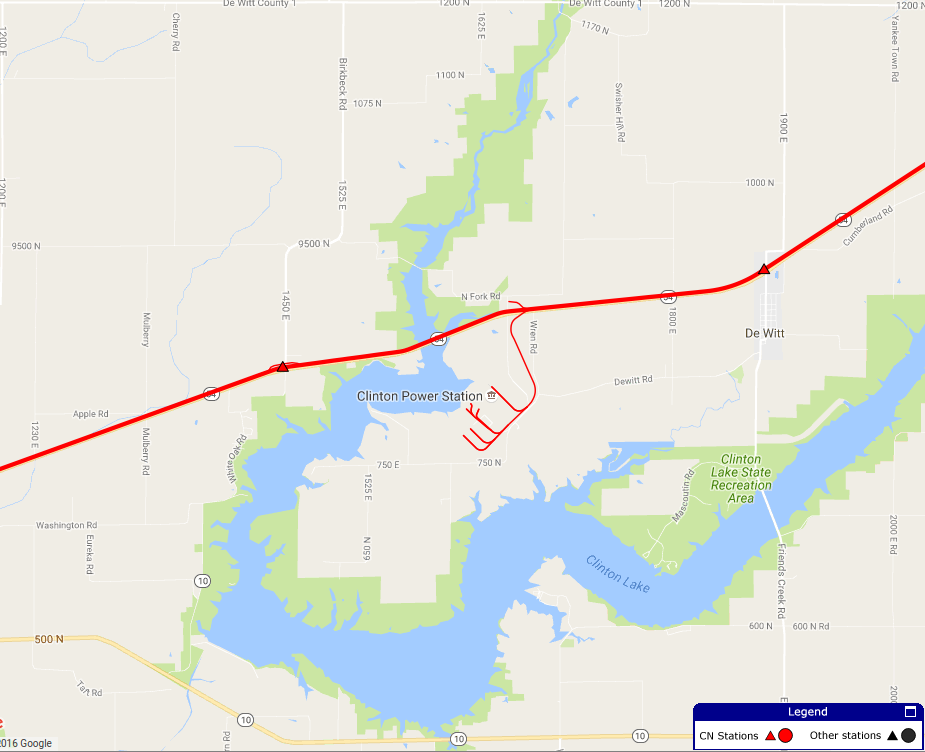
\includegraphics[width=0.8\columnwidth]{cnmap.png}	
        \caption{From \cite{canadian_national_railway_company_canadian_2016}, a map of Clinton Power Station in Clinton,IL
        with the Canadian National rail passing through.}
  \label{fig:cnmap}
\end{figure}

The proposed site's proximity to other power plants means that the transport
routes pass through fewer states and communities, which lessens the potential 
for conflict.

The capacity of the state to handle nuclear materials is also important.
The state of Illinois established a Division of Nuclear Safety in its \gls{IEMA}
which connects the state police and the Illinois Commerce Commission (ICC) to
 successfully transport 480 shipments of spent nuclear fuel since 1983
 \cite{iema_illinois_2005}. If a repository is built and operational, the already existing,
 experienced state organization will be able to handle the transportation logistics
 and security.  

In comparison, the 
transportation route to Yucca Mountain is identified to traverse 955 counties
with about 177 million persons, which is about 56\% of the US total
 \cite{halstead_yucca_2011}. \gls{SNF} transit is a sensitive topic to some states, and may
 demand reroutes that cause unexpected cost increases in transportation. Also,
 new railways would need to be constructed in order to ship the spent fuel inventories
 by rail. 


\begin{table}[h]
	\centering
        \caption {Site Access for Each Case}
	%\scalebox{0.60}{
		\begin{tabular}{|c|c|}
			\hline
			Case & Site Access \\
			\hline
			Case I & 0 \\
			Case II & 1 \\
			\hline
                \end{tabular}
                %}
\end{table}



\subsection{Expediency}

%get rid of this category or not? Since gov should purchase land from Exelon
% but could describe a smart way to do it (Exelon NWF exemption) and how it 
%outweighs downsides.

%federal: cost savings and less conflict with local community
			% the fact that is is a nuclear-town (Sweden example)
%local: less opposition and continuous flow of tax and jobs into the community

Leveraging existing infrastructure at an integrated site will allow for 
expedited acceptance of \gls{SNF} from temporary dry cask storage sites 
nationwide.

Dry casks are the result of the perpetual delay of a repository construction.
The proposed case would allow reactor sites to empty their spent fuel pools, which
would no longer necessitate dry storage campaigns. For example, Maine Yankee's 
\gls{ISFSI} cost was \$149.3 million in 2001 dollars, with an annual operating fee
of \$10 million per year \cite{lee_costing_2009}. 

The proposed case, once completed, will allow faster acceptance of \gls{SNF} and, 
accordingly, resumed collection of the \gls{NWF}, 
which will fund the repository operation and maintenance.

  The reference Yucca Mountain case does not require land purchase 
  because the land near Yucca Mountain is part of the Nevada Test Site. However, 
  it is lacking in infrastructure for \gls{SNF} handling.
  
  As mentioned previously, the licensed land area in the Clinton case is 
  sufficient to support a 70,000 \gls{MTHM} repository without purchase of land from 
  the public.  However, the federal government would need to purchase the 
  licensed area of the Clinton site from Exelon. Thus, the nuclear waste fee 
  would need to be leveraged toward paying Exelon for its land and the 
  facilities on site when Exelon shuts down the reactor.

  This would suggest a beneficial trade for both parties, since the government
  can purchase infrastructure and land simultaneously, and because Exelon can vastly
  save the cost of decommissioning by selling off the reactor site. The reactor
  core and power-generating component of the reactor site needs to be decommissioned,
  however. As a comparison, Maine Yankee, a \gls{PWR} with a capacity of 860MWe, had a
  decommissioning cost of 635 million \cite{aker_maine_2004}.


%%add maybe? or too much shade?
%Also, Clinton Power Plant, being a single unit power plant, has a much higher employee-per-GW ratio of 631, compared to, for example, 344 employee-per-GW at the Braidwood Power Plant, also in Illinois. %howtocitesinger With its inherent lack in efficiency for operation and maintenance, it would be an incentive for Exelon to host a repository to generate extra revenue. 

%clinton already has dry-cask infrastructure. 
%Utility: get rid of used facility without the trouble of decommissioning
%Federal: cost savings


The proposed case, being a once-operating nuclear power plant, has the facility to 
repack the spent fuel assemblies into a disposal cask. Its dry cask infrastructure 
is currently in use. However, this facility needs to be upgraded to increase its throughput, and should be preferably automatic, to minimize worker exposure. The transported spent fuel assemblies are repacked and inspected at the upgraded facility, and is sent to the emplacement tubes for final disposal. Not having to build an entirely new above-ground facility should greatly ease the consent-based process, for it seems like there would be minimal impact. 
 
The utility has a very high incentive since it will save on its decommissioning fee.
The construction of the repository next to the reactor site would substantially
reduce the cost of decommissioning, and it would not have to expand its dry storage
to empty out the pools. Exelon would be earning a profitable margin out of a
used nuclear power plant, which would otherwise be a cost burden to handle.

The base case requires a new above-ground facility, which not only costs a great
amount, but also will be considered problematic in the public's eye. 

%no specific advantage over the base case

% how to quanticize the incentive of emptying spent fuel storage pool?
% cost of dry cask installments for other plants (for stakeholders)
% security issue of Quad-Cities, Dresden and Lasalle and othereactors with elevated pool

%federal: able to resume collecting NWF
	% stop paying fines to utilities
%utility: cost savings in wet storage and dry cask infrastructure (security?)

A metric for expediency is then proposed which is inversely proportionate to 
the number of years until the federal government takes possession of the spent 
fuel. Estimating the likely timelines for each case is a challenge beyond the 
scope of this work. However, a bounding estimate can be derived from the time 
saved from use of existing infrastructure at the integrated facility. Avoiding 
that handling facility delay will save at least 5 years 
and likely much more on the timeline of Case II over that of Case I 
\cite{doe_strategy_2013}. Since the 
majority of \gls{SNF} would be destined for the eastern repository, in the combined case,
 approximately the same time savings could be assumed.

\begin{table}[h]
	\centering
        \caption {Expediency in Each Case}
	%\scalebox{0.60}{
		\begin{tabular}{|c|c|c|}
			\hline
                        Case & Time Saved [y] & NV \\
			\hline
			Case I & 0 & 0\\
			Case II & 5 & 1 \\
			\hline
                \end{tabular}
                %}
\end{table}

\section{Results and Discussion} 

To model the impact of these measures on the incentives of each stakeholder, 
the list of stakeholders considered follows in Table \ref{tab:stakeholders} 
alongside the weights indicating the magnitude of the importance of the incentive.
 
\begin{table}[h]
\centering
\caption {Metrics and Weight for Each Stakeholder}
\label{tab:stakeholders}
\scalebox{0.8}{
	\begin{tabular}{|l|c|c|c|c|}
	\hline
	Metric & Federal & State & Local & Utility  \\ \hline
	Transportation Burden & 3 & 2 & 1 & 1    \\ \hline
	Site Appropriateness & 3 & 2 & 1 & 1 \\ \hline
	Workforce Utilization & 3 & 2 & 2 & 2 \\ \hline
	Consenting Locals & 3 & 2 & 3 & 2 \\ \hline
	Site Access & 3 & 2 & 1 & 1 \\ \hline
	Expediency & 3 & 2 & 1 & 3 \\ \hline \hline
	Case I total & 3 &2 &1 & 1 \\ \hline
	Case II total & 16.9 & 11.2 & 7.9 & 9.2 \\ \hline
	\end{tabular}}
\end{table}

Results show that it is far more attractive for various stakeholders to 
site a repository at a non-operating nuclear power plant. Through strategical
siting, all the parties involved can benefit.

Given the current circumstances, a repository is crucial for the survival of nuclear
power. By siting one in a central location with sufficient licensed land,
a repository with sizable capacity can be built cheaper, more efficiently, and 
in a consent-based manner with the local community. 

   \section{Acknowledgments}

This material is based upon work supported by \gls{ACDIS}. Preliminary work was 
conducted in collaboration with the \gls{ISRG} within the \gls{NPRE}. The 
authors are accordingly grateful for guidance by Prof. Clifford Singer.




\bibliographystyle{ans}
\bibliography{bibliography}


\end{document}
